\documentclass[11pt,a4paper]{article}
\usepackage[T1]{fontenc}
\usepackage[utf8]{inputenc}
\usepackage[brazilian]{babel}
\usepackage{lmodern}
\usepackage[scaled=0.90]{helvet}
\usepackage{microtype}
\usepackage[a4paper,top=2.5cm,bottom=2.6cm,left=2.5cm,right=2.5cm,headheight=21.3pt,footskip=1.3cm]{geometry}
\usepackage{graphicx}
\usepackage{xcolor}
\usepackage{booktabs}
\usepackage{tabularx}
\usepackage{longtable}
\usepackage{array}
\usepackage{enumitem}
\usepackage{amssymb}
\usepackage{titlesec}
\usepackage{fancyhdr}
\usepackage{caption}
\usepackage{framed}
\usepackage{float}
\usepackage[hidelinks]{hyperref}

\definecolor{navy}{HTML}{1F3A5F}
\definecolor{navy2}{HTML}{2D5283}
\definecolor{accent}{HTML}{B5651D}
\definecolor{ink}{HTML}{1B2430}
\definecolor{ink2}{HTML}{4A5566}
\definecolor{ink3}{HTML}{7B8696}
\definecolor{rule}{HTML}{E3E0D8}
\definecolor{paper}{HTML}{FBFAF7}
\definecolor{ok}{HTML}{2F6B3C}
\definecolor{warn}{HTML}{9A6A00}

\color{ink}
\linespread{1.06}
\setlength{\parskip}{0.45em}
\setlength{\parindent}{0pt}

\titleformat{\section}{\sffamily\Large\bfseries\color{navy}}{\thesection}{0.6em}{}
\titlespacing*{\section}{0pt}{2.4ex plus .6ex minus .2ex}{1.1ex}
\titleformat{\subsection}{\sffamily\large\bfseries\color{ink}}{\thesubsection}{0.55em}{}
\titlespacing*{\subsection}{0pt}{1.8ex plus .4ex}{0.7ex}
\titleformat{\subsubsection}{\sffamily\bfseries\color{ink2}}{\thesubsubsection}{0.5em}{}

\captionsetup{font={small,sf},labelfont={bf,color=accent},labelsep=period,skip=6pt}
\captionsetup[table]{position=top}

\pagestyle{fancy}
\fancyhf{}
\renewcommand{\headrulewidth}{0.4pt}
\renewcommand{\headrule}{\hbox to\headwidth{\color{rule}\leaders\hrule height \headrulewidth\hfill}}
\fancyhead[L]{\sffamily\footnotesize\color{ink3}Patentometria --- guia passo a passo}
\fancyhead[R]{\sffamily\footnotesize\color{ink3}\thepage}

\renewenvironment{leftbar}{%
  \def\FrameCommand{{\color{accent}\vrule width 2.6pt}\hspace{10pt}}%
  \MakeFramed{\advance\hsize-\width\FrameRestore}}%
 {\endMakeFramed}

\newenvironment{nota}[1][Nota]%
 {\begin{leftbar}\small\color{ink2}\textbf{\textsf{\color{accent}#1.}}\ }%
 {\end{leftbar}}

\newenvironment{alerta}[1][Cuidado]%
 {\begin{leftbar}\small\color{ink2}\textbf{\textsf{\color{warn}#1.}}\ }%
 {\end{leftbar}}

\newcolumntype{L}{>{\raggedright\arraybackslash}X}
\newcolumntype{R}{>{\raggedleft\arraybackslash}X}
\newcommand{\campo}[1]{\texttt{\small #1}}
\newcommand{\num}[1]{\textsf{\textbf{#1}}}
\newcommand{\marcador}{\textcolor{ok}{$\blacksquare$}}
\renewcommand{\arraystretch}{1.15}
\setlist[enumerate]{leftmargin=1.5em,itemsep=3pt,topsep=3pt}
\setlist[itemize]{leftmargin=1.4em,itemsep=3pt,topsep=3pt}

\begin{document}
\begin{titlepage}
\thispagestyle{empty}
{\color{navy}\rule{\linewidth}{2.5pt}}\\[1.0cm]
{\sffamily\footnotesize\color{ink3}PATENTOMETRIA \; · \; ANÁLISE DESCRITIVA DE PATENTES}\\[0.35cm]
{\sffamily\bfseries\fontsize{31}{35}\selectfont\color{navy} Guia passo a passo}\\[0.35cm]
{\sffamily\Large\color{ink2} Como usar e interpretar cada tela}\\[1.4cm]

\begin{leftbar}
\small\color{ink2}
Este guia percorre a aplicação da primeira rodada até a leitura dos indicadores. Cada passo tem
quatro blocos fixos: \textbf{Objetivo} (o que se quer obter), \textbf{O que fazer} (a sequência de
cliques), \textbf{Como interpretar} (o que cada número e cada campo significam) e
\textbf{Checkpoint} (como saber que o passo terminou certo).
\end{leftbar}

\vspace{0.6cm}
{\sffamily\small\color{ink2}
\textbf{Dados de demonstração.} As telas deste guia vêm de um estudo sintético sobre sensores ópticos
aplicados a amostras ambientais, com quatro exportações de bases diferentes. O fluxo resultante é
conhecido e serve de referência: \num{15} documentos identificados, \num{2} modelos de utilidade
excluídos, \num{13} documentos elegíveis e \num{5} famílias após a deduplicação. Nenhum número aqui
descreve um mercado real.}\\[0.8cm]
{\sffamily\small\color{ink3}
Versão da aplicação: 0.4.1 \quad · \quad Rodada de referência: 15/10/2026 \quad · \quad
Capturas: outubro de 2026}\\[0.3cm]
{\color{navy}\rule{\linewidth}{0.8pt}}
\end{titlepage}

\section*{Como usar este guia}
\addcontentsline{toc}{section}{Como usar este guia}

O trabalho tem seis abas, na ordem em que devem ser percorridas: \textbf{Coleta e consolidação},
\textbf{Ligações}, \textbf{Nomes}, \textbf{Famílias e triagem}, \textbf{Indicadores} e
\textbf{VOSviewer}. As abas \textbf{Importar} e \textbf{Planilha base} ficam à direita e servem para
entrar e sair com os dados.

Cada passo deste guia corresponde a uma decisão metodológica, não apenas a uma tela. A leitura correta
é sempre a mesma: primeiro entenda \emph{o que está sendo contado} (documento, família, atribuição),
depois \emph{qual é o denominador}, e só então compare o número com outra rodada ou com outro estudo.

\begin{nota}[A regra dos três números]
Todo indicador desta aplicação responde a três perguntas: qual é a unidade (documento? família?
depositante?), qual é o denominador (quantas famílias têm o dado?) e qual é a data de corte (a coleta).
Um percentual sem essas três informações não deve ser citado em texto.
\end{nota}

\tableofcontents
\clearpage
\section{Passo 1 — Abrir a aplicação e criar o estudo}
\label{sec:passo1}

\subsection*{Objetivo}
Criar o \emph{estudo}, que guarda a configuração metodológica e todas as rodadas de busca de um mesmo
trabalho. O estudo é o contêiner; nada é calculado antes de existir uma rodada com arquivos.

\begin{figure}[H]
\centering
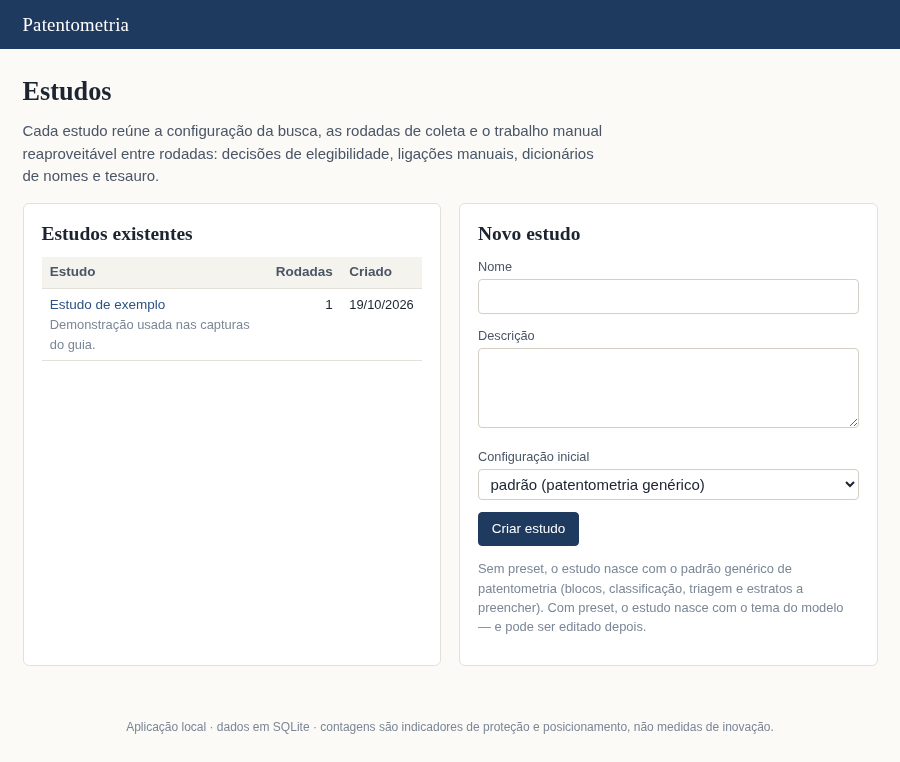
\includegraphics[width=0.95\linewidth]{img/01_home.png}
\caption{Tela inicial com a lista de estudos. No ambiente de demonstração existe um único estudo,
criado com o preset de exemplo.}
\label{fig:home}
\end{figure}

\subsection*{O que fazer}
\begin{enumerate}
\item Abra a aplicação (o instalador a inicia em \campo{http://127.0.0.1:8080}).
\item Confira se o estudo já existe na lista. Se existir, clique no nome.
\item Se não existir, preencha \textbf{Nome}, uma \textbf{Descrição} curta e escolha o preset
      \campo{vazio.json}.
\item Clique em \textbf{Criar estudo} e abra o estudo recém-criado.
\end{enumerate}

\subsection*{Como interpretar}
A lista mostra, para cada estudo, quantas rodadas ele tem. \textbf{Um estudo sem rodada é apenas um
formulário}: a configuração ainda não foi aplicada a nenhum corpus.

O nome deve identificar o recorte, não a instituição: ``Sensores ópticos em amostras ambientais'' é
melhor que ``Estudo 1''. A descrição é livre, mas vale registrar a pergunta que o estudo responde ---
ela será a chave para interpretar os indicadores depois.

\begin{nota}[Por que separar estudo e rodada]
A mesma pergunta pode ser respondida com buscas diferentes (bases diferentes, datas diferentes). Se
tudo ficasse em um único registro, não haveria como comparar duas coletas. A rodada é a foto datada;
o estudo é a regra do jogo.
\end{nota}

\begin{alerta}[Erro comum]
Criar um estudo novo para cada nova busca. Isso fragmenta o histórico. O correto é criar uma
\emph{rodada} dentro do mesmo estudo (Passo 3).
\end{alerta}

\subsection*{Checkpoint}
\marcador\; O estudo aparece na tela inicial e, ao abrir, mostra o painel com \textbf{0 rodadas}.

\section{Passo 2 — Configurar o estudo}
\label{sec:passo2}

\subsection*{Objetivo}
Definir o contrato metodológico: o que conta como tema, o que conta como contexto, quais períodos
serão comparados, como a triagem será feita e quais estratos existirão.

\begin{figure}[H]
\centering
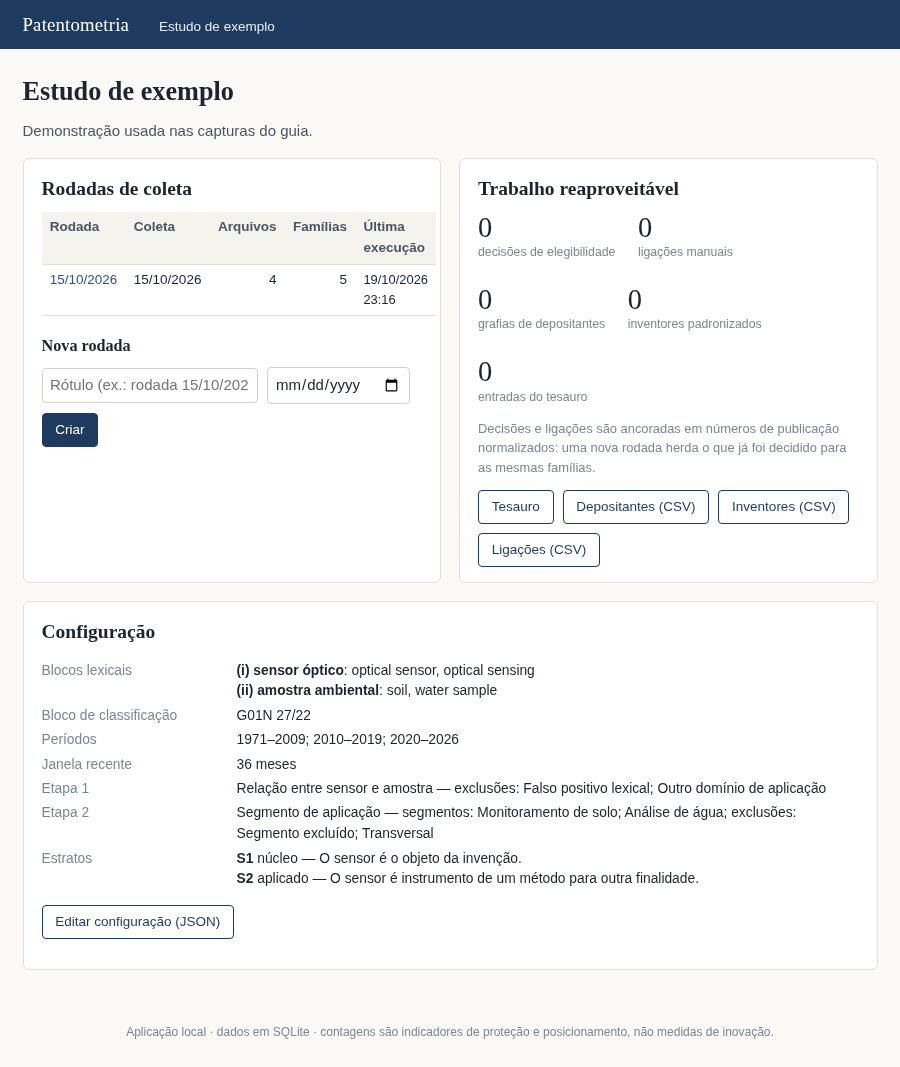
\includegraphics[width=0.72\linewidth]{img/02_estudo.png}
\caption{Painel do estudo com o resumo da configuração: blocos lexicais, classificação, períodos,
janela, categorias de triagem e estratos. O botão \emph{Editar configuração (JSON)} abre o editor.}
\label{fig:config}
\end{figure}

\subsection*{O que fazer}
\begin{enumerate}
\item Abra \textbf{Configuração} no painel do estudo.
\item Ajuste os campos do JSON (a aplicação valida antes de salvar).
\item Use \textbf{Ver tesauro} para conferir os sinônimos que serão aplicados na leitura dos títulos.
\item Clique em \textbf{Salvar} e confira o resumo que aparece no topo.
\end{enumerate}

\subsection*{Como interpretar}
Cada chave tem um efeito verificável:

\begin{itemize}
\item \campo{blocks}: grupos de termos usados para destacar o título e o resumo na triagem. O bloco
      (i) é o tema; o bloco (ii) é o contexto de aplicação. Termo genérico demais aumenta o ruído;
      termo específico demais deixa famílias fora.
\item \campo{classification\_block}: códigos de classificação usados como filtro de leitura. Não
      substituem a consulta feita na base; servem para checar aderência.
\item \campo{periods}: faixas de ano de anterioridade. Precisam ser crescentes e não se sobrepor;
      o último período é sempre parcial e deve ser lido com essa ressalva.
\item \campo{window\_months}: janela de comparação usada nos indicadores de tendência.
\item \campo{stage1}/\campo{stage2}: rótulos e motivos de exclusão. Os motivos viram categorias no
      PRISMA --- escreva poucos e mutuamente exclusivos.
\item \campo{strata}: camadas analíticas com definição textual. A definição é o que permite a outra
      pessoa repetir a classificação.
\end{itemize}

\begin{nota}[A matriz de campos]
Logo abaixo do editor, a aplicação mostra quais campos cada base exporta. Um traço não significa
zero: significa que aquela base não informa o campo. Todo indicador construído sobre um campo parcial
carrega essa lacuna, e o denominador exibido na tela é a forma de torná-la visível.
\end{nota}

\begin{alerta}[Erro comum]
Copiar a configuração de outro estudo sem revisar os blocos. Os termos de um tema não descrevem outro,
e a triagem inteira herda o erro.
\end{alerta}

\subsection*{Checkpoint}
\marcador\; O resumo no topo mostra os dois blocos, os três períodos e os dois estratos, e o botão de
validação não aponta erro.

\section{Passo 3 — Criar a rodada e enviar as exportações}
\label{sec:passo3}

\subsection*{Objetivo}
Registrar uma coleta datada e carregar nela os arquivos exportados de cada base.

\begin{figure}[H]
\centering
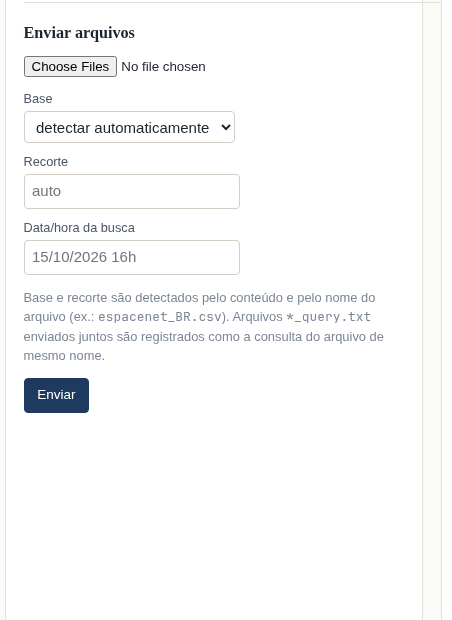
\includegraphics[width=0.62\linewidth]{img/03_upload_painel.png}
\caption{Formulário de envio de arquivos, na própria tela da rodada. O nome do arquivo define a
base e o recorte; a data de execução registra quando a busca foi feita.}
\label{fig:upload}
\end{figure}

\subsection*{O que fazer}
\begin{enumerate}
\item No estudo, clique em \textbf{Nova rodada} e informe um rótulo (por exemplo, a data da coleta).
\item Envie os arquivos de uma vez. O nome deve seguir o padrão \campo{<base>\_<recorte>.csv} ou
      \campo{.txt}: \campo{lens\_nucleo.csv}, \campo{espacenet\_nucleo.csv},
      \campo{google\_nucleo.csv}, \campo{darwent\_nucleo.txt}.
\item Se a exportação não trouxer a consulta no cabeçalho, envie também
      \campo{lens\_query.txt} com o texto da consulta.
\item Informe a data/hora de execução e confirme o envio.
\end{enumerate}

\subsection*{Como interpretar}
Cada arquivo se torna um registro com três informações: \textbf{base} (lens, espacenet, google,
darwent, inpi), \textbf{recorte} (o conjunto; \campo{nucleo} é o principal) e \textbf{número de
registros lidos}. A aplicação ignora arquivos de ``concepts'' e arquivos fora do padrão --- se um
arquivo não aparecer na lista, o problema é o nome.

O recorte não é decoração: a consolidação usa apenas o recorte definido em \campo{core\_recorte}. Um
arquivo nomeado com outro recorte entra no estudo, mas fica fora da base unificada.

\begin{nota}[Proveniência]
Guardar a consulta permite responder ``de onde veio este número?'' meses depois. A tela de rodada
marca com aviso as exportações sem consulta declarada; isso não impede o cálculo, mas impede a
reprodutibilidade.
\end{nota}

\begin{alerta}[Erro comum]
Reenviar arquivos na mesma rodada sem marcar \textbf{substituir}. Os documentos são somados e o
PRISMA passa a contar duplicatas que não são famílias.
\end{alerta}

\subsection*{Checkpoint}
\marcador\; A rodada lista quatro arquivos e o total de registros lidos é \num{15}.

\section{Passo 4 — Consolidar e ler o fluxo PRISMA}
\label{sec:passo4}

\subsection*{Objetivo}
Transformar documentos de bases diferentes em famílias comparáveis e medir quanto do volume inicial
era redundância.

\begin{figure}[H]
\centering
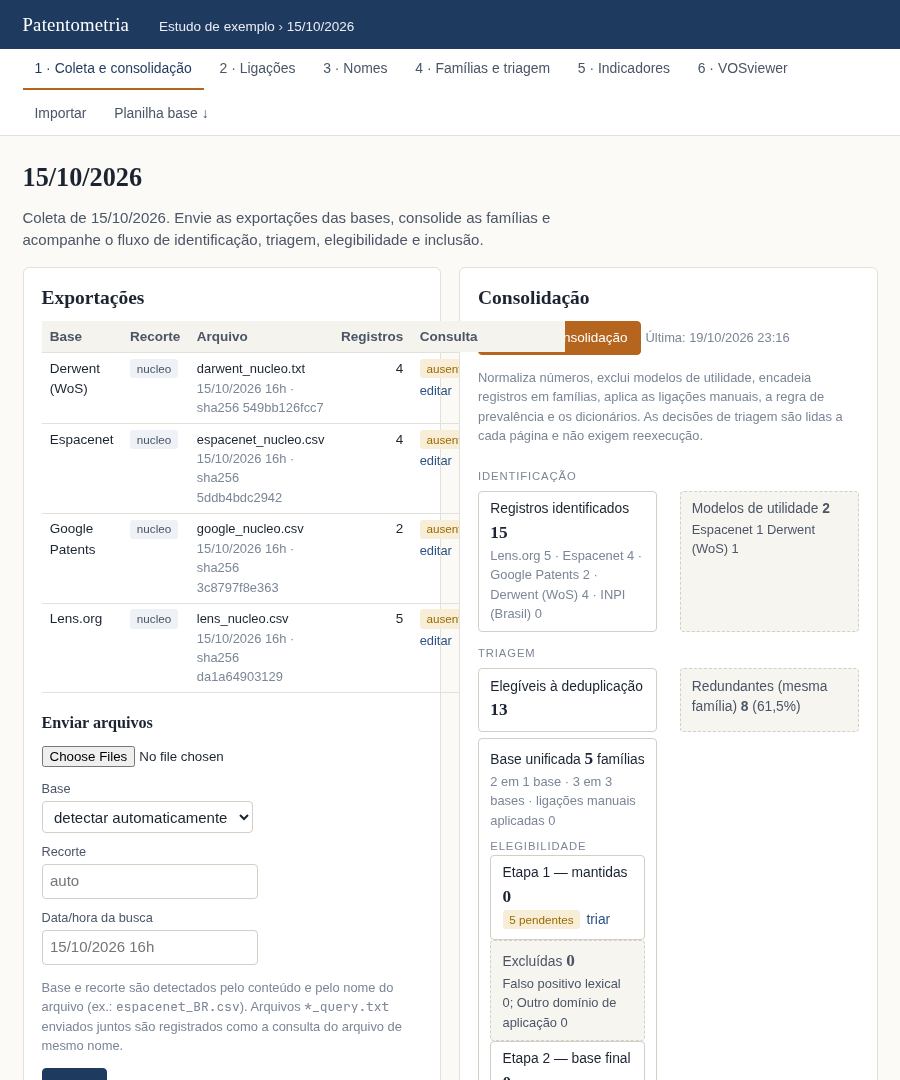
\includegraphics[width=0.8\linewidth]{img/04_rodada_topo.png}
\caption{Fluxo da rodada de demonstração: 15 documentos identificados, 2 modelos de utilidade
excluídos, 13 elegíveis e 5 famílias. O painel também mostra a distribuição por número de bases e o
que ainda está pendente na triagem.}
\label{fig:prisma}
\end{figure}

\subsection*{O que fazer}
\begin{enumerate}
\item Na rodada, clique em \textbf{Consolidar}.
\item Leia o fluxo de cima para baixo, conferindo cada subtotal.
\item Abra \textbf{Famílias} para ver o resultado da deduplicação.
\end{enumerate}

\subsection*{Como interpretar}
\begin{itemize}
\item \textbf{Identificados (15)}: documentos lidos, somando as quatro bases (5 + 4 + 2 + 4).
\item \textbf{Modelos de utilidade (2)}: documentos excluídos por tipo, antes da deduplicação.
\item \textbf{Elegíveis (13)}: identificados menos os excluídos por tipo.
\item \textbf{Redundantes (8, 61,5\%)}: documentos que representam invenções já contadas em outra
      família ou em outra base. É a medida do retrabalho que a deduplicação elimina.
\item \textbf{Base unificada (5)}: famílias efetivamente analisadas. O texto auxiliar mostra a
      distribuição: \num{3} famílias aparecem em três bases e \num{2} em apenas uma.
\item \textbf{Pendentes (5)}: famílias ainda sem decisão na etapa 1. Enquanto houver pendente, a
      base final não existe.
\end{itemize}

A distribuição por número de bases é um indicador de cobertura, não de qualidade: uma família
presente em três bases é mais robusta a erro de exportação; uma família exclusiva de uma base pode ser
uma lacuna das outras buscas. As exclusivas aparecem discriminadas por base --- na demonstração, uma
do Google e uma do Derwent.

\begin{nota}[Como citar o PRISMA]
Cite sempre o conjunto completo: ``15 documentos identificados, 2 excluídos por tipo, 13 elegíveis,
8 redundantes (61,5\%) e 5 famílias''. Dizer apenas ``5 famílias'' esconde o esforço de deduplicação e
impede a comparação com outras rodadas.
\end{nota}

\begin{alerta}[Erro comum]
Tratar ``famílias'' como ``patentes''. Uma família pode reunir pedido e concessão, em vários países;
contar documentos em vez de famílias infla qualquer série histórica.
\end{alerta}

\subsection*{Checkpoint}
\marcador\; Identificados $-$ modelos de utilidade $=$ elegíveis; elegíveis $-$ redundantes $=$ famílias;
e o número de pendentes da etapa 1 é igual ao número de famílias.

\section{Passo 5 — Triagem, etapa 1: a família trata do tema?}
\label{sec:passo5}

\subsection*{Objetivo}
Decidir, família por família, se o documento mantém relação com o tema e o contexto definidos no
estudo. É a etapa que separa volume de corpus.

\begin{figure}[H]
\centering
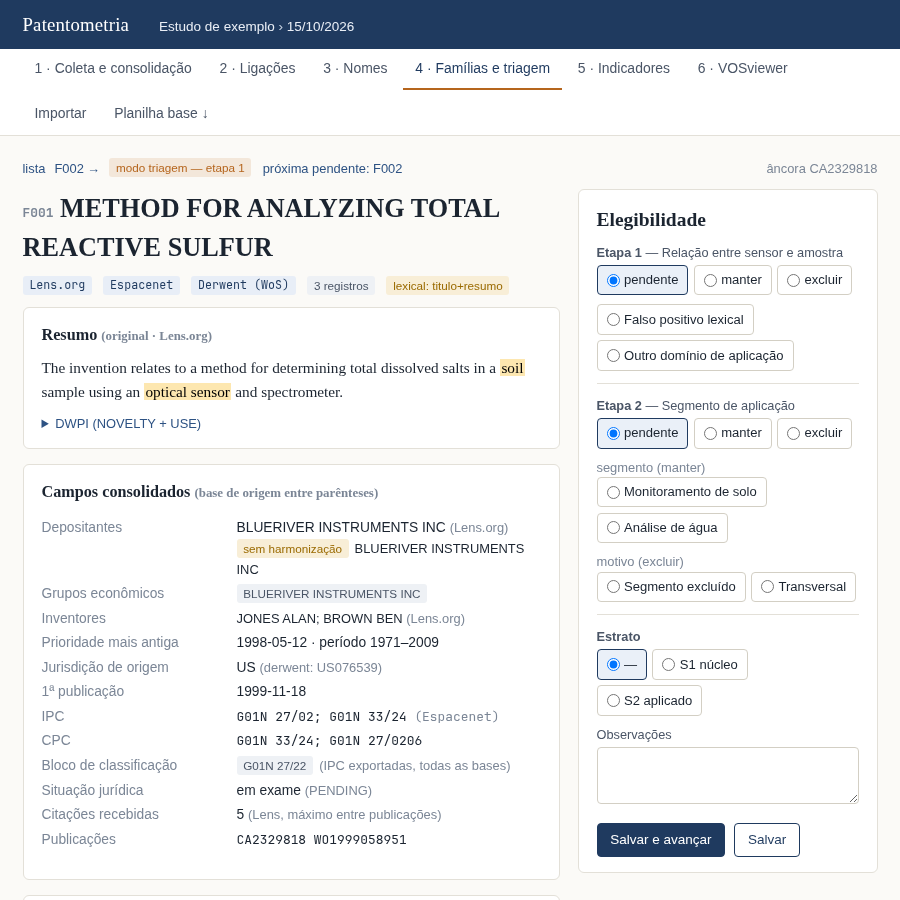
\includegraphics[width=0.78\linewidth]{img/08_triagem_topo.png}
\caption{Ficha de triagem. À esquerda, título e resumo com os termos dos blocos destacados e os dados
consolidados da família; à direita, o painel de decisão.}
\label{fig:triagem1}
\end{figure}

\subsection*{O que fazer}
\begin{enumerate}
\item Na rodada, clique em \textbf{Triar} (etapa 1). A aplicação abre a primeira família pendente.
\item Leia título e resumo com os destaques. Confira depositantes, prioridade e classificações.
\item Marque \textbf{Manter} ou \textbf{Excluir}. Ao excluir, escolha o motivo na lista.
\item Use \textbf{Salvar e próxima} para registrar e seguir. Repita até não haver pendentes.
\end{enumerate}

\subsection*{Como interpretar}
O destaque mostra onde os termos dos blocos aparecem. Um destaque no título é mais forte que um
destaque no resumo; um destaque isolado, sem relação semântica, é o típico falso positivo lexical.

A decisão é da \emph{família}, não do documento: o objetivo é não contar a mesma invenção duas vezes.
Três leituras ajudam a manter consistência:

\begin{itemize}
\item \textbf{Relação com o tema}: o tema é o objeto da invenção ou apenas uma palavra no texto?
\item \textbf{Relação com o contexto}: a aplicação declarada está no contexto do estudo?
\item \textbf{Evidência suficiente}: título e resumo bastam para decidir? Se não, use a ficha completa
      (Passo 9) antes de marcar.
\end{itemize}

\begin{nota}[O que ``manter'' significa]
Manter na etapa 1 não é incluir no corpus final: é admitir a família na etapa 2 (segmento) e na
classificação por estrato. A exclusão, ao contrário, é definitiva para esta rodada e alimenta os
motivos do PRISMA.
\end{nota}

\begin{alerta}[Erro comum]
Decidir pelo número de citações. Citação mede visibilidade na base, não aderência ao tema; uma família
muito citada pode ser justamente um falso positivo.
\end{alerta}

\subsection*{Checkpoint}
\marcador\; O contador de pendentes da etapa 1 chega a zero e o PRISMA passa a mostrar mantidas e
excluídas com seus motivos.

\section{Passo 6 — Triagem, etapa 2, e classificação por estrato}
\label{sec:passo6}

\subsection*{Objetivo}
Classificar as famílias mantidas por segmento de aplicação e por estrato analítico, produzindo a base
final do estudo.

\begin{figure}[H]
\centering
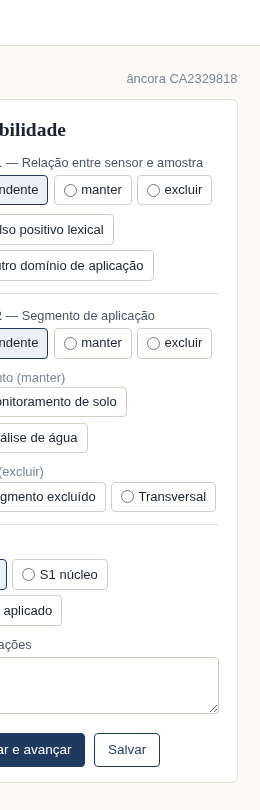
\includegraphics[width=0.4\linewidth]{img/08_triagem_painel.png}
\caption{Painel de decisão da ficha, recortado: etapa 1, etapa 2, estrato e observações.}
\label{fig:triagem2}
\end{figure}

\subsection*{O que fazer}
\begin{enumerate}
\item Clique em \textbf{Triar etapa 2}. Só aparecem as famílias mantidas na etapa 1.
\item Escolha o \textbf{segmento} de aplicação e, se houver, o motivo de exclusão da etapa 2.
\item Atribua o \textbf{estrato} (S1, S2, conforme a definição do estudo).
\item Registre observações quando a decisão não for óbvia; elas ficam na planilha.
\end{enumerate}

\subsection*{Como interpretar}
A etapa 2 responde ``para que serve a invenção?''; o estrato responde ``qual é o papel do tema na
invenção?''. São perguntas diferentes e não devem ser confundidas.

Na demonstração, S1 é ``o sensor é o objeto da invenção'' e S2 é ``o sensor é instrumento de um método
para outra finalidade''. A definição textual importa: sem ela, dois avaliadores classificam o mesmo
documento de formas diferentes.

\begin{nota}[Por que estratificar]
A média do corpus mistura invenções de naturezas distintas. Separar S1 e S2 permite comparar, por
exemplo, depositantes que protegem o componente e depositantes que protegem o método de uso --- e
evita conclusões sobre ``o setor'' a partir de populações heterogêneas.
\end{nota}

\begin{alerta}[Erro comum]
Deixar o estrato em branco e seguir para os indicadores. A base final fica incompleta e os gráficos
por estrato perdem parte das famílias sem aviso.
\end{alerta}

\subsection*{Checkpoint}
\marcador\; O PRISMA mostra a base final com o total de incluídas e a distribuição por estrato; não há
pendentes nas etapas 1 e 2.

\section{Passo 7 — Ligações manuais entre registros}
\label{sec:passo7}

\subsection*{Objetivo}
Corrigir os casos em que a deduplicação automática não reconheceu a mesma invenção em bases
diferentes, ou em que reconheceu duas invenções como uma.

\begin{figure}[H]
\centering
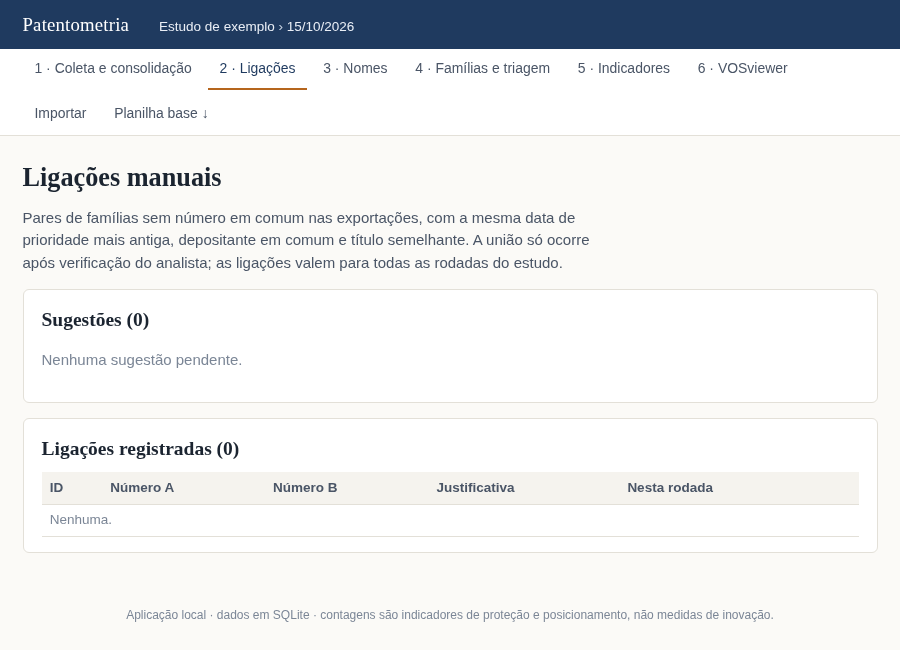
\includegraphics[width=0.9\linewidth]{img/09_ligacoes.png}
\caption{Tela de ligações no estado inicial: nenhuma sugestão e nenhuma ligação registrada. Quando há
pares suspeitos, eles aparecem nesta lista com os números e o motivo.}
\label{fig:ligacoes}
\end{figure}

\subsection*{O que fazer}
\begin{enumerate}
\item Abra \textbf{Ligações}. Leia a lista de sugestões: pares com mesma prioridade, mesmo depositante
      ou título muito próximo.
\item Para cada par, clique em \textbf{Aceitar} (é a mesma família) ou \textbf{Rejeitar} (não é).
\item Se o par não aparecer na lista, registre manualmente os dois números.
\item Volte à rodada e clique em \textbf{Consolidar} novamente para aplicar as ligações.
\end{enumerate}

\subsection*{Como interpretar}
A deduplicação automática usa regras conservadoras: prioridade mais antiga, depositante normalizado e
semelhança de título. Ela erra nos dois sentidos --- deixa de unir famílias quando a prioridade não foi
exportada e une demais quando dois pedidos compartilham prioridade sem serem a mesma invenção.

Aceitar uma ligação \emph{reduz} o número de famílias; rejeitar \emph{aumenta}. Por isso a tela mostra
as ligações aplicadas e as sem correspondência: um número grande de sem correspondência costuma
indicar número digitado errado ou formato de publicação diferente entre bases.

\begin{nota}[Ligação é decisão de estudo]
As ligações valem para o estudo inteiro, não para uma rodada. Ao repetir a coleta, elas continuam
valendo; revise-as quando o corpus mudar de escopo.
\end{nota}

\begin{alerta}[Erro comum]
Editar a ligação e não reconsolidar. Sem a reconsolidação, o PRISMA continua com os números antigos e
a decisão parece não ter efeito.
\end{alerta}

\subsection*{Checkpoint}
\marcador\; O número de famílias muda depois da reconsolidação e as ligações aparecem como ``aplicadas''.

\section{Passo 8 — Harmonizar depositantes e inventores}
\label{sec:passo8}

\subsection*{Objetivo}
Transformar nomes exportados (grafias diferentes, subsidiárias, traduções) em identificadores
consistentes, para que a contagem por depositante faça sentido.

\begin{figure}[H]
\centering
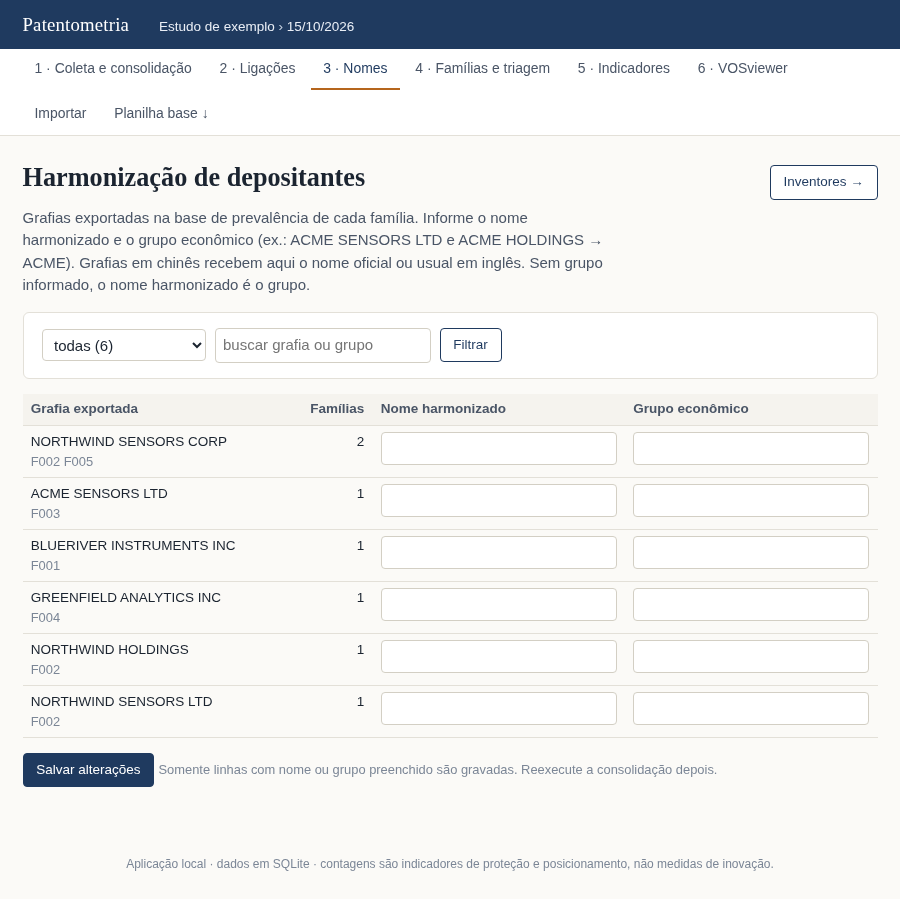
\includegraphics[width=0.72\linewidth]{img/10_depositantes.png}
\caption{Harmonização de depositantes: cada grafia exportada aparece com o número de famílias, um
campo de nome harmonizado e um campo de grupo econômico.}
\label{fig:depositantes}
\end{figure}

\subsection*{O que fazer}
\begin{enumerate}
\item Abra \textbf{Nomes} e escolha \textbf{Depositantes}.
\item Para cada grafia, preencha o \textbf{nome harmonizado} (a forma que você vai citar) e o
      \textbf{grupo econômico}, quando houver controladora comum.
\item Use o filtro para trabalhar por família de grafias.
\item Clique em \textbf{Salvar alterações} e reconsolide a rodada.
\item Repita em \textbf{Inventores}, com atenção a abreviações e homônimos.
\end{enumerate}

\subsection*{Como interpretar}
A tela separa três conceitos que costumam ser confundidos:

\begin{itemize}
\item \textbf{Grafia exportada}: o que a base entregou, sem tratamento.
\item \textbf{Nome harmonizado}: a forma única usada nas tabelas e nos textos.
\item \textbf{Grupo econômico}: a controladora que reúne várias pessoas jurídicas.
\end{itemize}

O número ao lado da grafia é o de \emph{famílias} em que ela aparece. Depois da harmonização, o
indicador de concentração passa a somar famílias por grupo, e não por grafia --- é isso que evita
concluir que um mercado é fragmentado quando, na verdade, são três subsidiárias do mesmo grupo.

\begin{nota}[Atribuições, não famílias]
Uma família com dois depositantes conta para os dois. Por isso a soma das colunas pode ser maior que o
número de famílias. A tela de indicadores informa o total de atribuições justamente para tornar essa
diferença visível.
\end{nota}

\begin{alerta}[Erro comum]
Preencher grupo econômico sem nome harmonizado. A aplicação só grava linhas com nome ou grupo
preenchido; sem harmonização, a grafia original continua sendo a unidade de contagem.
\end{alerta}

\subsection*{Checkpoint}
\marcador\; As grafias relevantes têm nome harmonizado, os grupos estão preenchidos e os indicadores, após
reconsolidar, mostram menos depositantes do que grafias.

\section{Passo 9 — Ler a lista e a ficha de uma família}
\label{sec:passo9}

\subsection*{Objetivo}
Conferir o que a consolidação produziu: quais famílias existem, quantas bases as sustentam e quais
dados foram consolidados em cada uma.

\begin{figure}[H]
\centering
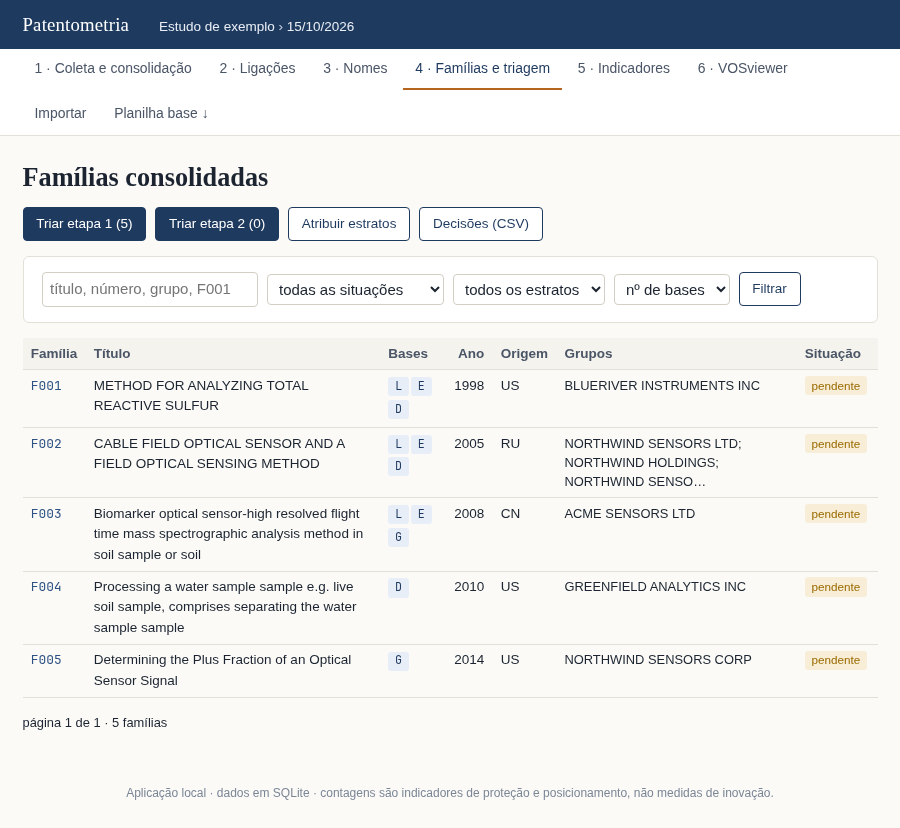
\includegraphics[width=0.82\linewidth]{img/06_familias.png}
\caption{Lista de famílias da rodada, com chave, título, número de bases, documentos e situação na
triagem.}
\label{fig:familias}
\end{figure}

\begin{figure}[H]
\centering
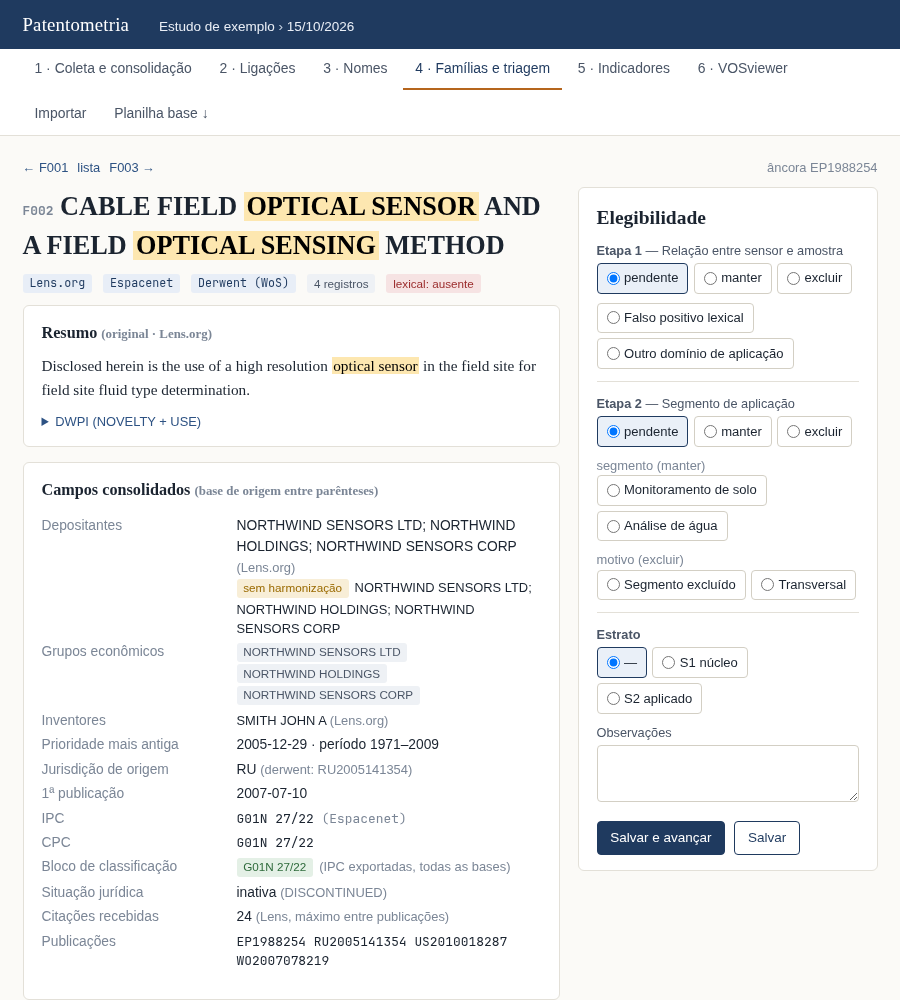
\includegraphics[width=0.75\linewidth]{img/07_familia_topo.png}
\caption{Ficha da família F002: dados consolidados, título e resumo com destaques, e os registros
originais de cada base.}
\label{fig:familia}
\end{figure}

\subsection*{O que fazer}
\begin{enumerate}
\item Abra \textbf{Famílias} e ordene pela coluna que interessa (bases, documentos, chave).
\item Clique em uma família para abrir a ficha.
\item Confira os dados consolidados e abra a lista de registros originais.
\item Se houver divergência entre bases, registre na observação da triagem.
\end{enumerate}

\subsection*{Como interpretar}
A chave (\campo{F001}, \campo{F002}) é interna e serve para navegar; não é um identificador de patente.
O \textbf{número de bases} mostra a cobertura; o número de \textbf{documentos} mostra quantos registros
foram agrupados naquela família.

Na ficha, os campos consolidados vêm de regras de precedência: o título original da família, a
prioridade mais antiga, o conjunto de depositantes e as classificações. Quando as bases divergem, a
aplicação escolhe um valor e mantém os originais visíveis --- a divergência é informação, não erro a
ser apagado.

\begin{nota}[Registro original é a fonte]
Sempre que um número parecer estranho, volte ao registro original. Título traduzido, resumo truncado
e prioridade ausente são as três causas mais comuns de discordância entre bases.
\end{nota}

\begin{alerta}[Erro comum]
Usar a chave interna em uma citação. Em texto, cite o número de publicação ou a prioridade; a chave
muda a cada rodada.
\end{alerta}

\subsection*{Checkpoint}
\marcador\; Você consegue explicar, para uma família qualquer, quantos documentos ela tem, de quais bases
e qual é a prioridade mais antiga.

\section{Passo 10 — Indicadores descritivos}
\label{sec:passo10}

\subsection*{Objetivo}
Descrever o corpus por período, jurisdição, concentração de titularidade, depositantes, inventores,
classificação, anterioridade e citações.

\begin{figure}[H]
\centering
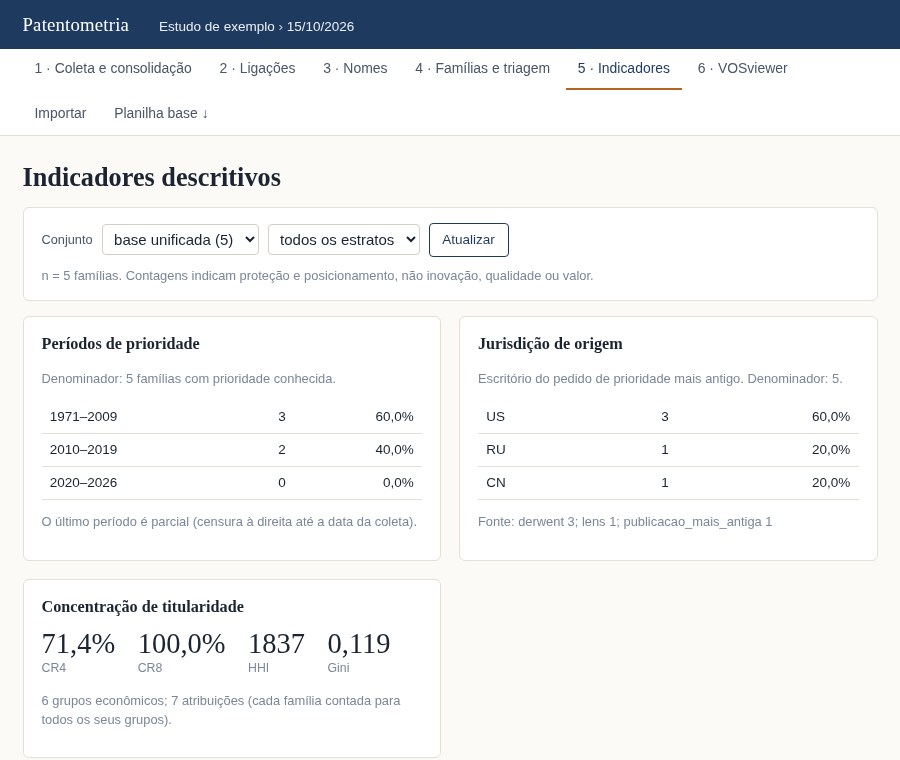
\includegraphics[width=0.92\linewidth]{img/12_indicadores_1.png}
\caption{Indicadores: períodos de prioridade, jurisdição de origem e concentração de titularidade.
Todos os cartões informam o denominador.}
\label{fig:ind1}
\end{figure}

\begin{figure}[H]
\centering
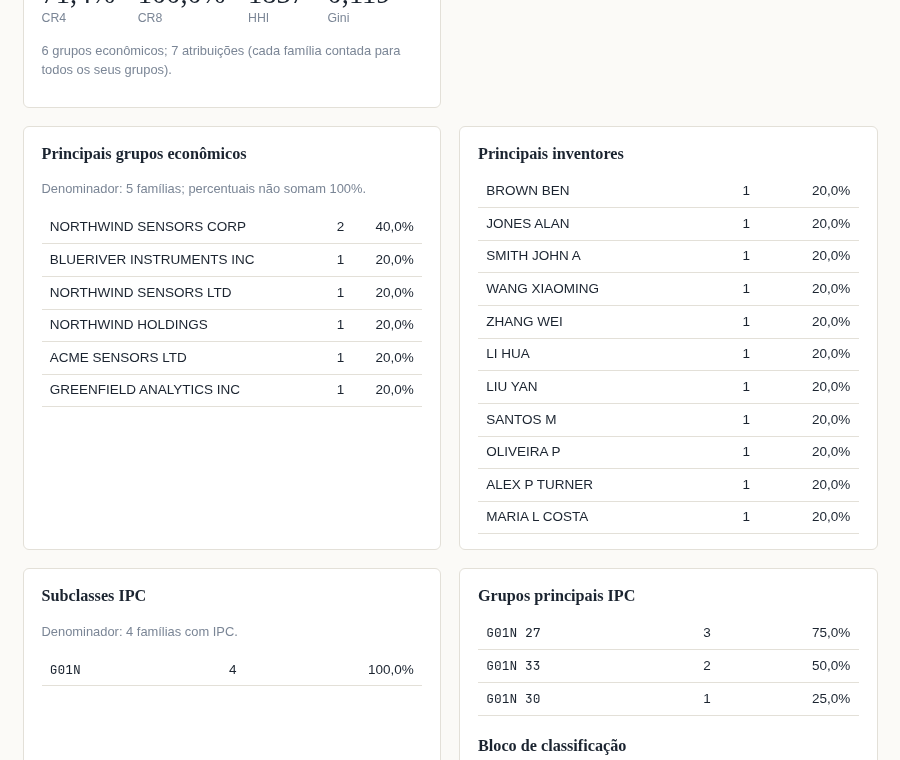
\includegraphics[width=0.92\linewidth]{img/12_indicadores_2.png}
\caption{Depositantes, grupos econômicos e inventores, com o número de famílias e de atribuições.}
\label{fig:ind2}
\end{figure}

\begin{figure}[H]
\centering
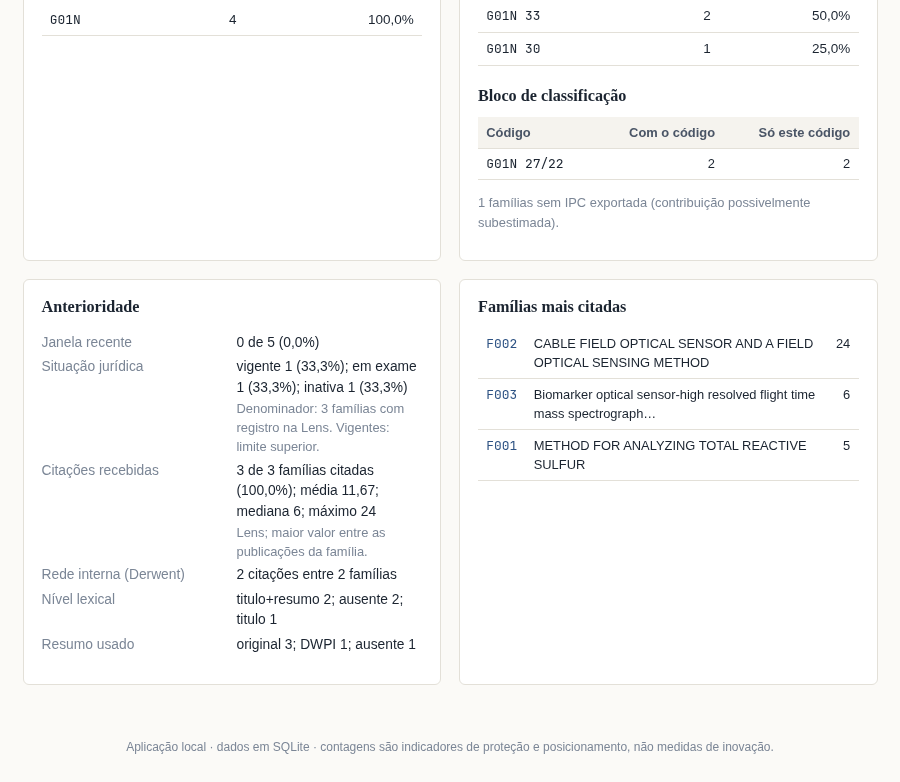
\includegraphics[width=0.92\linewidth]{img/12_indicadores_3.png}
\caption{Classificação IPC, anterioridade e famílias mais citadas.}
\label{fig:ind3}
\end{figure}

\subsection*{O que fazer}
\begin{enumerate}
\item Abra \textbf{Indicadores} e escolha o conjunto: \emph{base unificada} ou \emph{base final}.
\item Escolha o estrato (todos, S1, S2).
\item Leia cada cartão começando pelo denominador; só depois compare os valores.
\item Exporte a planilha base (Passo 12) para guardar os números com a data da coleta.
\end{enumerate}

\subsection*{Como interpretar}
\textbf{Períodos.} Na demonstração, 3 famílias (60\%) têm prioridade entre 1971 e 2009, 2 (40\%) entre
2010 e 2019 e nenhuma entre 2020 e 2026. O último período é parcial: a censura à direita faz qualquer
queda parecer maior do que é.

\textbf{Jurisdição.} Conta o escritório da prioridade mais antiga: EUA 3 (60\%), Rússia 1, China 1. É
um indicador de onde a proteção foi pedida primeiro, não de onde o mercado é maior.

\textbf{Concentração.} CR4 = 71,4\%, CR8 = 100\%, HHI = 1.837 e Gini = 0,119, sobre 6 grupos
econômicos e 7 atribuições. CR4 e CR8 medem a fatia dos maiores; HHI cresce quando poucos concentram;
Gini mede desigualdade na distribuição. Com cinco famílias, esses valores são instáveis: um único
documento muda o resultado. Use-os para descrever o corpus, não para afirmar estrutura de mercado.

\textbf{Depositantes e inventores.} O número entre parênteses é de famílias; a soma das atribuições
pode exceder o total de famílias porque uma família pode ter vários titulares. Compare sempre com o
total informado no rodapé do cartão.

\textbf{IPC.} Uma família pode ter várias classificações; por isso a soma das classes não fecha com o
número de famílias. A classe principal é a mais frequente, não a única.

\textbf{Anterioridade.} Mostra o tempo entre a prioridade e a publicação (ou a coleta). Serve para
separar pedidos recentes de famílias consolidadas; não mede velocidade de inovação.

\textbf{Top citadas.} Citações recebidas na base de origem. Bases diferentes cobrem citações de formas
diferentes; o ranking é interno ao corpus e não é comparável entre estudos.

\begin{nota}[Como escrever o resultado]
Use a fórmula ``X de Y famílias (Z\%)\!'', com o recorte e a data: ``3 de 5 famílias (60\%) tinham
prioridade anterior a 2010, na coleta de 15/10/2026''. Sem Y e sem a data, o número não é verificável.
\end{nota}

\begin{alerta}[Erro comum]
Ler CR4 ou HHI como prova de concentração de mercado. O indicador descreve a titularidade do corpus
selecionado; a seleção da busca já é uma escolha metodológica.
\end{alerta}

\subsection*{Checkpoint}
\marcador\; Para cada indicador citado, você sabe dizer a unidade, o denominador e a data de corte.

\section{Passo 11 — Gerar o pacote para o VOSviewer}
\label{sec:passo11}

\subsection*{Objetivo}
Exportar o corpus da base final em formato compatível com o VOSviewer e importar de volta o mapa e a
rede para guardar o resultado junto do estudo.

\begin{figure}[H]
\centering
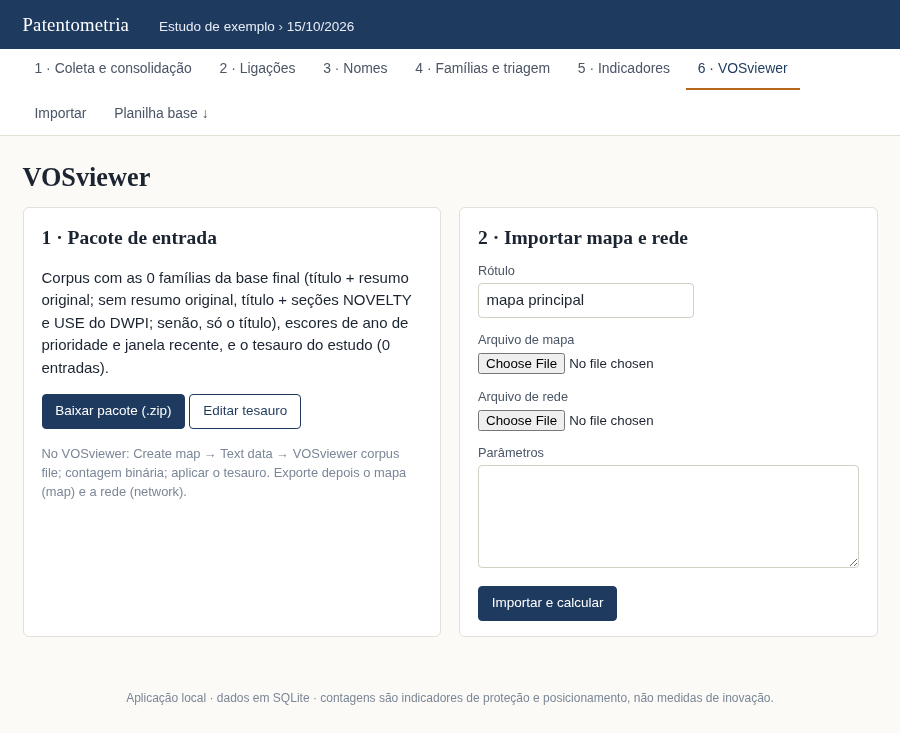
\includegraphics[width=0.9\linewidth]{img/13_vosviewer.png}
\caption{Tela do VOSviewer: geração do pacote de entrada e importação do mapa e da rede já calculados
no programa externo.}
\label{fig:vos}
\end{figure}

\subsection*{O que fazer}
\begin{enumerate}
\item Abra \textbf{VOSviewer} e clique em \textbf{Baixar pacote (.zip)}.
\item No VOSviewer, crie o mapa a partir do arquivo de corpus (Create map $\rightarrow$ Text data).
\item Exporte o mapa e a rede e importe os dois arquivos na aplicação.
\item Descreva os parâmetros usados no campo de observações.
\end{enumerate}

\subsection*{Como interpretar}
O pacote contém título e resumo de cada família da base final, os anos de prioridade e o tesauro do
estudo. Isso significa que o mapa reflete \emph{apenas} o que passou pela triagem --- se a base final
estiver vazia, o corpus sai vazio (é o que acontece na demonstração antes da triagem).

No VOSviewer, a escolha do tipo de análise muda a pergunta: coocorrência de termos descreve o discurso
do corpus; coautoria descreve redes de inventores; citação descreve proximidade entre documentos. O
número mínimo de ocorrências e o tamanho do cluster precisam ser informados no guia do estudo, porque
mudam o desenho.

\begin{nota}[Mapa é exploratório]
Cluster não é categoria analítica validada. Use o mapa para levantar hipóteses e volte aos documentos
para confirmar; não cite o cluster como se fosse um achado.
\end{nota}

\begin{alerta}[Erro comum]
Rodar o VOSviewer na base unificada e apresentar o mapa como se fosse a base final. Os dois conjuntos
respondem a perguntas diferentes.
\end{alerta}

\subsection*{Checkpoint}
\marcador\; O pacote foi gerado, o mapa e a rede estão anexados ao estudo e os parâmetros usados estão
registrados.

\section{Passo 12 — Planilha base, importação e encerramento}
\label{sec:passo12}

\subsection*{Objetivo}
Sair do aplicativo com os dados em formato aberto e com o estudo reprodutível por outra pessoa.

\begin{figure}[H]
\centering
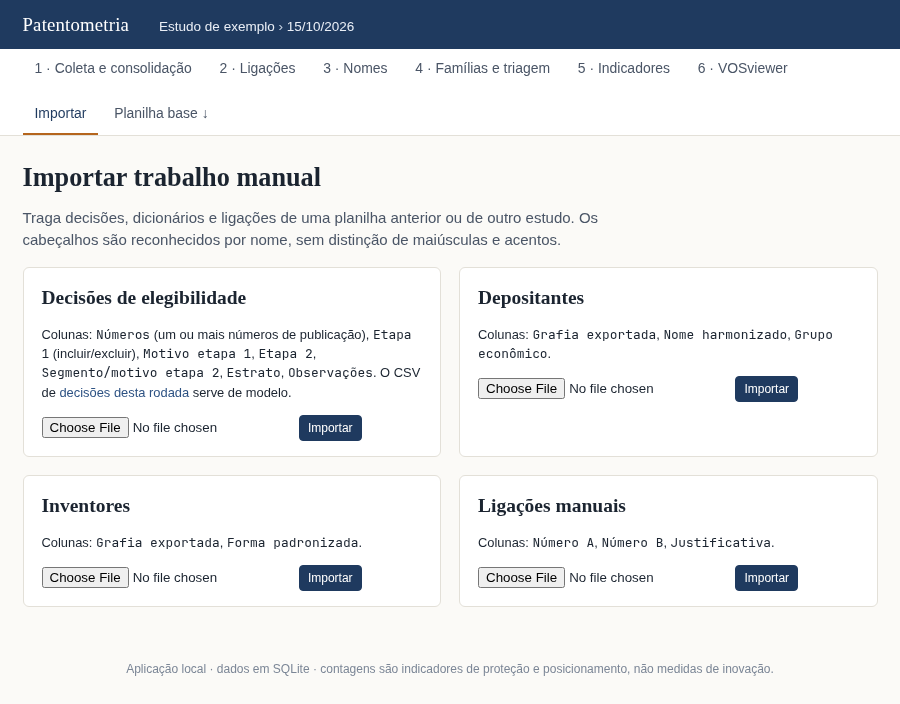
\includegraphics[width=0.9\linewidth]{img/14_importar.png}
\caption{Tela de importação: entrada de um estudo ou de uma planilha já preparada, com validação antes
de gravar.}
\label{fig:importar}
\end{figure}

\subsection*{O que fazer}
\begin{enumerate}
\item Clique em \textbf{Planilha base} para baixar o \campo{.xlsx} com famílias, decisões e indicadores.
\item Clique em \textbf{Decisões} para baixar o CSV com o rastro da triagem.
\item Em \textbf{Importar}, use o JSON exportado do estudo para reproduzi-lo em outra máquina.
\item Guarde a pasta de dados (banco e arquivos) junto do projeto.
\end{enumerate}

\subsection*{Como interpretar}
A planilha é a camada de auditoria: cada linha é uma família, com os campos consolidados e as decisões.
O CSV de decisões é o que permite reconstruir o PRISMA sem reabrir a aplicação.

O JSON de estudo contém a configuração, não os dados. Importar o JSON em outra instalação recria as
regras; os arquivos das bases precisam ser reenviados para reproduzir os números.

\begin{nota}[Checklist de encerramento]
\num{1)} PRISMA fechado e conferido; \num{2)} nenhuma família pendente nas etapas 1 e 2;
\num{3)} depositantes e inventores harmonizados; \num{4)} ligações aplicadas e reconsolidadas;
\num{5)} indicadores lidos com denominador e data; \num{6)} planilha e decisões exportadas;
\num{7)} backup da pasta de dados.
\end{nota}

\begin{alerta}[Erro comum]
Exportar a planilha antes da última reconsolidação. O arquivo nasce com os números do momento em que
foi gerado --- confira a data no cabeçalho.
\end{alerta}

\subsection*{Checkpoint}
\marcador\; Você consegue entregar a pasta do estudo com configuração, exportações, planilha, decisões e
backup, e outra pessoa consegue repetir a rodada seguindo este guia.

\section{Glossário curto}
\label{sec:glossario}

\begin{tabularx}{\linewidth}{@{}p{4.1cm}L@{}}
\toprule
\textbf{Termo} & \textbf{O que significa nesta aplicação} \\
\midrule
Documento & Registro de uma patente ou pedido em uma base (uma publicação). \\
Família & Conjunto de documentos que protegem a mesma invenção; é a unidade de contagem da base unificada. \\
Base unificada & Todas as famílias da rodada, depois de deduplicar os documentos entre as bases. \\
Base final & Subconjunto que passou pelas etapas de triagem e pelos estratos. \\
Estrato & Camada analítica definida no estudo (por exemplo, núcleo e aplicado). \\
Atribuição & Cada vínculo entre uma família e um depositante, inventor ou classificação; uma família pode ter vários. \\
CR4 / CR8 & Soma da participação dos quatro (ou oito) maiores depositantes. \\
HHI & Soma dos quadrados das participações; varia de 0 a 10.000. \\
Gini & Desigualdade na distribuição entre depositantes; 0 é igualdade perfeita. \\
Anterioridade & Data do depósito mais antigo que sustenta a família. \\
\bottomrule
\end{tabularx}

\section{Problemas comuns}
\label{sec:problemas}

\subsection*{O arquivo foi ignorado na importação}
O nome precisa indicar base e recorte: \campo{lens\_nucleo.csv}, \campo{espacenet\_BR.csv},
\campo{darwent\_nucleo.txt}. Arquivos com ``concepts'' no nome são descartados de propósito.

\subsection*{O aviso ``sem consulta declarada'' não sai}
Cada exportação pode trazer a consulta no cabeçalho (Espacenet e Google) ou em um arquivo
\campo{<base>\_query.txt}. Sem isso, a rodada perde a proveniência: você sabe o resultado, mas não
consegue repetir a busca.

\subsection*{Os números do PRISMA não fecham}
Identificados menos modelos de utilidade deve ser igual a elegíveis. Se não for, verifique se algum
arquivo foi importado duas vezes na mesma rodada (use \campo{--substituir} ao reimportar).

\subsection*{A tela de indicadores está vazia}
Confira o seletor de conjunto: \emph{base unificada} mostra todas as famílias; \emph{base final} só
mostra o que passou pela triagem. Sem decisões, a base final tem zero famílias.

\subsection*{O VOSviewer importou um corpus vazio}
O pacote usa a base final. Se a triagem ainda não foi concluída, o arquivo sai sem famílias --- o que
é um aviso, não um erro de exportação.

\end{document}
